\chapter{Tests and Results}
\label{chapter:tests}

In this chapter, several experiments will be performed in order to assess the quality and features of technologies and developed application. The main goals are: to obtain an empiric and realistic conclusion on which technology serves better the purpose of this thesis and to assess how the application fares when subject to different stress tests.

This chapter will be divided in two different sections: one regarding the comparison between Bluetooth and Wi-Fi Direct in Android devices, via different tests and other regarding the tests performed with the developed application, to better understand where it performs better and worse, proving or not if the theoretical choices made translate into actual performance gains.

\section{Bluetooth vs. Wi-Fi Direct in Android Devices}

This section will cover the differences, advantages and disadvantages of both Bluetooth and Wi-Fi Direct. A series of experiments will be conducted and their results analysed, providing a justification on which technology is best suited for this application and applications with a similar architecture and/or purpose.

Since the first implementation of Bluetooth in Android, several releases have been developed. Different Bluetooth versions provide different \gls{QoS}, this may impact the performed tests, as a device running a newer Bluetooth version may provide better results than a device running an older version. To avoid confusion, all the tested devices will be running Bluetooth version 4.0.

The tests will range from communication distances to data rates analysis, and most of the tests will be backed up by both theoretical and empirical results, although in some cases, due to the inability of getting precise measures, the results will be taken from previously developed works.

\subsection{Ranges of Communication}
\label{subsec:ranges}

The ranges of communication of both technologies are of extreme importance. They can reduce or increase greatly the number of hops a packet has to pass through, in order to reach the destination. If the range of communication is too short, the number of connections made will increase, this may cause an overload of the network, and the deterioration of the communication medium. On the other hand, if the communication range is long, the devices are able to jump through bigger hops, creating less traffic in the network and establishing the least possible number of connections.

Both technologies share some similarities: they depend on the environment of the communication, \textit{i.e.}, the elements that are surrounding the devices and possible obstacles in the way. The experiments were conducted, for the obstacle experiment, in a corridor of Torre Norte in the vicinities of Instituto Superior Técnico and, for the line-of-sight experiment in the outside area of Instituto Superior Técnico. It is important to note that although this experiments were made with as little interference as possible, there are certain elements that are impossible to controls, such as wireless communications from other devices and metal objects, such as metal lockers and cars.

Bluetooth establishes four different classes for the devices that may use this technology, depending on the transmitting power. Mobile phones are inserted in class 2 and, for that class, the specified average range of transmission in order to have a reliable connection is \textit{10m}, from \cite{bluetooth}.

Wi-Fi Direct on the other hand offers, theoretically, ranges of communication up to, approximately, \textit{200m}, from \cite{wfdrange}, which poses for a much better solution, in terms of network off-loading and general depth.

In order to verify these claims from both technologies, two mobile devices were taken to an open space, although with some limitations as described above, and several searches were made, until the devices stopped being discovered by one another.

It is expected that the measured distances are smaller than the theoretical ones, as the environment affects the experiments results, due to multipath fading, path loss, attenuation and interference from other devices.

Bluetooth was able to create a connection between devices from a distance up to \textit{42m} apart, see Figure \ref{fig:btMaxVisib} for the overall scheme of this experiment. This value is bigger than what was expected judging by the theoretical value of \textit{10m}, although the health of the connection was not verified - see Subsection \ref{subsec:normalftdr} to see how the distance affects the data rates. Using Wi-Fi Direct the devices were able to communicate from a maximum distance of \textit{77m}, see Figure \ref{fig:wfdMaxVisib} for the overall scheme of this experiment, which is, considerably, smaller than the theoretical value of \textit{200m}.

\begin{figure}[ht]
   \noindent\makebox[\textwidth]
    {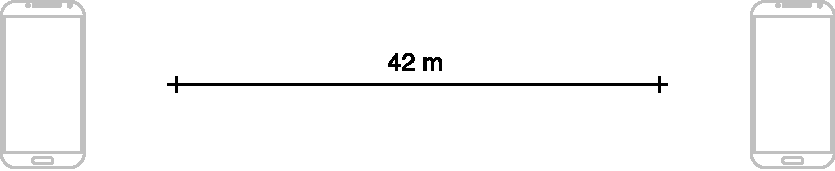
\includegraphics[width=0.8\textwidth]{images/bt_max_visib.pdf}}
	\caption{\label{fig:btMaxVisib} Max range of Bluetooth communication with line-of-sight between devices}
\end{figure}

\begin{figure}[ht]
   \noindent\makebox[\textwidth]
    {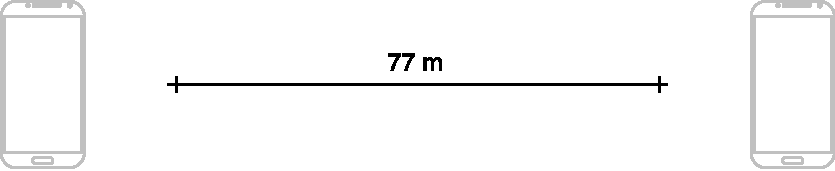
\includegraphics[width=0.8\textwidth]{images/wfd_max_visib.pdf}}
	\caption{\label{fig:wfdMaxVisib} Max range of Wi-Fi Direct communication with line-of-sight between devices}
\end{figure}

Both tests were made with a direct line-of-sight between devices. For the next ones there will be obstacles in the way of communication. It is expected that this affects greatly the communication ranges. The first test was made using Bluetooth technology where a wall was blocking the line-of-sight between devices, see Figure \ref{fig:btMaxInv}. The second test was made using Wi-Fi Direct, and, in order to maintain the same environment as the previous experiment, to get reliable results, it was situated in the same place as the first, see Figure \ref{fig:wfdMaxInv}. However, due to the environment configuration, it was impossible to recreate the experiment with only one wall, so two walls are now dividing the devices. Since the walls introduce a loss in the signal power, the more walls are between devices, the bigger the losses will be.

\begin{figure}[ht]
   \noindent\makebox[\textwidth]
    {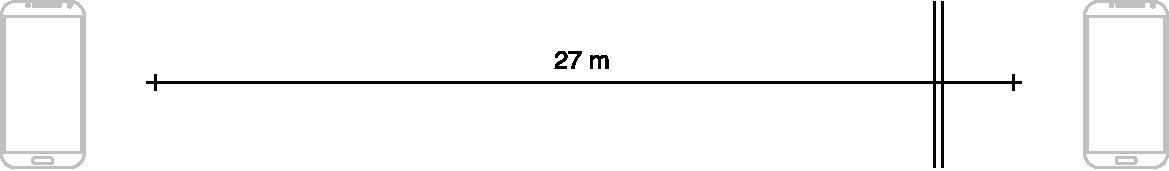
\includegraphics[width=0.8\textwidth]{images/bt_max_inv.pdf}}
	\caption{\label{fig:btMaxInv} Max range of Bluetooth communication without line-of-sight between devices}
\end{figure}

\begin{figure}[ht]
   \noindent\makebox[\textwidth]
    {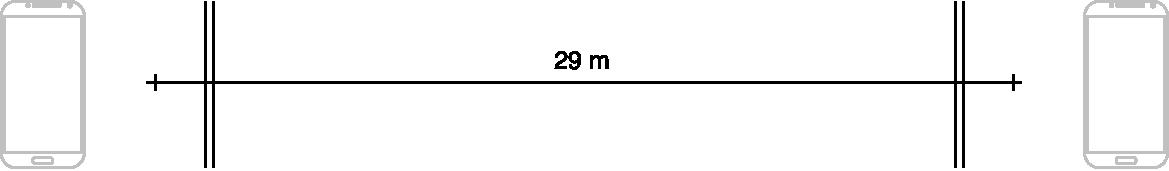
\includegraphics[width=0.8\textwidth]{images/wfd_max_inv.pdf}}
	\caption{\label{fig:wfdMaxInv} Max range of Wi-Fi Direct communication without line-of-sight between devices}
\end{figure}

As expected the obstacle, in this case the wall, created a significant decrease on the maximum range of communication. The devices were able to communicate via Bluetooth from a distance of \textit{27m}, closer to the theoretical \textit{10m}.

Wi-Fi Direct was also able to communicate from a smaller maximum distance, measuring \textit{29m} with the signal passing through both walls. From a smaller distance, it was verified that this technology could communicate with only wall in the way, meaning it also surpasses Bluetooth when an obstacle is in the way of communication.

After these experiments, it is possible to conclude that Wi-Fi Direct is more desirable, since it provides better coverage than Bluetooth to similar areas. Also, there is no evidence that Wi-Fi Direct suffers more losses from obstacles, maintaining its desirability. This was already to expect, both from the theoretical values and from the transmission powers\footnote{Transmission powers impact directly the range of transmission, since they affect the signal strength, a crucial characteristic for receivers to better capture the transmissions. A bigger transmit power, usually, creates a bigger signal strength leading to the signal being capture over bigger distances, as referred in \cite{txpower}, for instance.}, since Bluetooth is mostly known for its lower transmit powers, if compared to Wi-Fi.

\subsection{Discovery Times}
\label{subsec:normaldisc}

The discovery time is a critical factor for this work. The discovery process is one of the biggest time consumers during an application run. Thus, minimizing it, is a great advantage for the overall performance of the application.

For the purpose of testing the Bluetooth and Wi-Fi Direct discovery times, three mobile devices were used: Samsung Grand Neo, running Android version 4.2.2; Motorola Moto G2, running Android version 7.1; Huawei P8 Lite, running Android version 6.0, providing an heterogeneous sample space.

Every device is running Bluetooth version 4.0, as previously stated. This Bluetooth version theoretically provides a discovery time of \textit{10.24s}, as mentioned in \cite{bluetoothspec}, \cite{btdisc1} and \cite{btdisc2}. To confirm this hypothesis, discovery times values from the three devices were measured. Each device was submitted to multiple discoveries with a different number of discovered peers, ranging from 0 to 3 peer devices found.

Figure \ref{fig:normaldisc} shows the measured Bluetooth discovery times from the three tested devices. It is important to note that these results were measured with a chronometer, having a maximum precision of \textit{0.5s}.

Samsung Grand Neo (in blue) is constant throughout the measuring, having a Bluetooth discovery time of \textit{13s}. Motorola Moto G2 (in green) shows some variance in the various measurements. The Bluetooth discovery time measures range from \textit{13s} to \textit{14s}, having an average of \textit{13.85s}. Huawei P8 Lite (in purple) shows the biggest deviation throughout the sample space. Its Bluetooth discovery time measures range from \textit{16.5s} to \textit{15s}, having an average of \textit{15.976s}.

\begin{figure}[ht]
	\noindent\makebox[\textwidth]
	{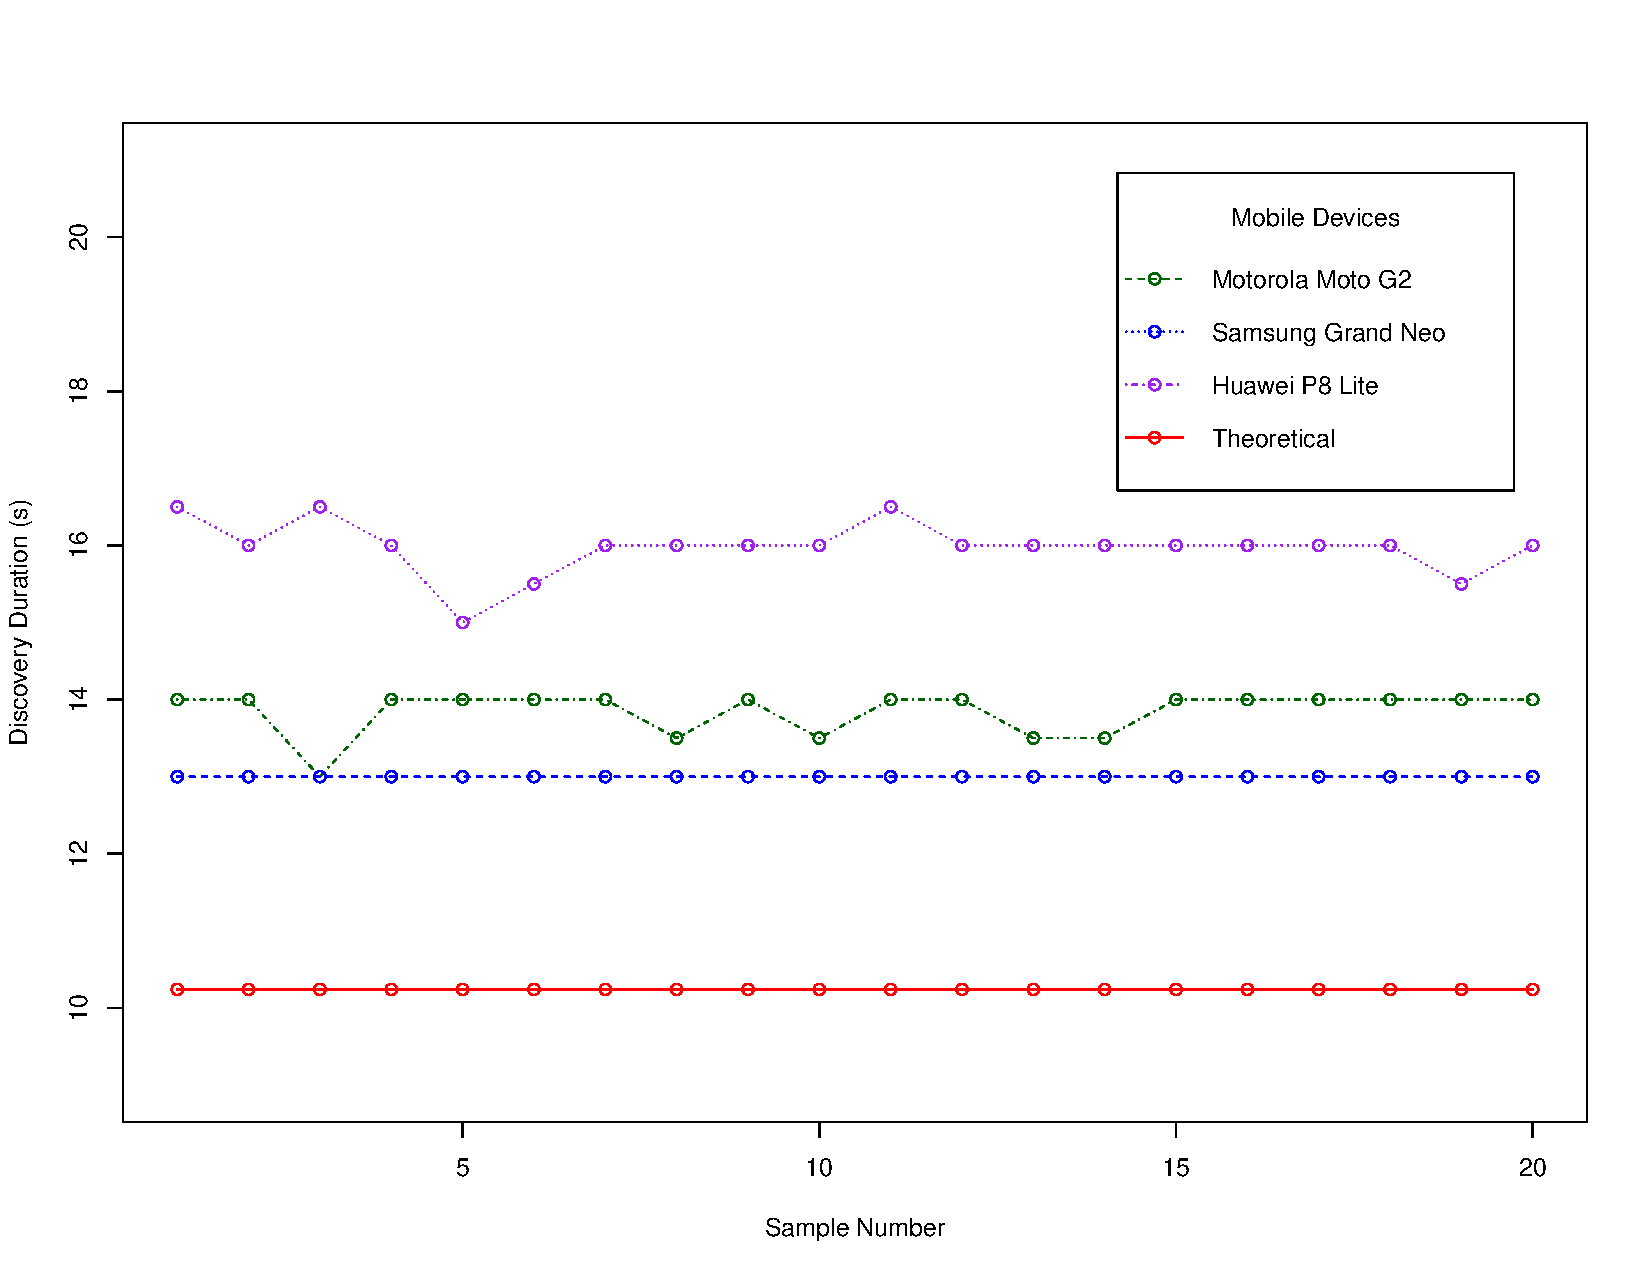
\includegraphics[width=1.2\textwidth]{images/plot_normal_disc.pdf}}
	\caption{\label{fig:normaldisc} Plot of the measured Bluetooth discovery times from the three devices.}
\end{figure}

None of the three devices approached the theoretical Bluetooth discovery time value of \textit{10.24s}, the difference is quite significant in a delay-sensitive application, such as the developed one.

Each device showed a different average Bluetooth discovery time, this difference in the discovery times can be due to the different hardware used in the devices, since each device is produced by a different manufacturer.

Wi-Fi Direct on the other hand does not provide a discovery time limit. This technology is constantly scanning for peer devices, until the user stops the ongoing search - see \cite{wfddisc}. This is also a cause of Wi-Fi Direct's bigger energy consumption, since this process is running in background when the technology is being used.

However, it is possible to program an application limiting the discovery period of Wi-Fi Direct. This provides a more flexible discovery time than Bluetooth's, since it can be tweaked according the application's purpose.

\subsection{Throughput}
\label{subsec:normalftdr}

In this subsection the data rates of both Bluetooth and Wi-Fi Direct will be analysed and compared. Since the data rates are technology specific, instead of conducting experiments that may not provide the most accurate results, a paper will be described, containing appropriate and accurate tests to these technologies' throughputs.

Bluetooth version 4.0 provides a theoretical, maximum throughput of \textit{24Mbps}, from \cite{bluetoothspec}, whereas Wi-Fi Direct provides a maximum throughput of \textit{250Mbps}, as stated in \cite{wfdrate}. To provide a precise measurement of both Bluetooth and Wi-Fi Direct's actual throughput in Android devices, the work developed by A. Mtibaa \textit{et al.} in \cite{throughputpaper} will be described. 

The devices used were two Google Nexus 5 smartphones running Android version 4.4.4, with Bluetooth 4.0. These devices were tested in three distinct environments: indoor line-of-sight, in an underground walkway \textit{350m} long and \textit{10m} wide. Indoor with obstacles, consisting of a set of offices separated by walls, \textit{4m} apart. Outdoor line-of-sight, in an outdoor walkway with \textit{582m} long and \textit{8m} wide.

Two sets of three experiments were conducted: one in each environment, using both communication technologies. In each experiment the throughput was measured by establishing a \gls{TCP} connection beetween client and server and sending \textit{5MB} files. The server then measured the total number of received bytes over \textit{2s} intervals, computing the throughput in that period.

In Figure \ref{fig:btthroughput} it is possible to see the measured devices' throughput, using Bluetooth, in the three described environments, as a function of the distance between devices.

Figure \ref{fig:btin} shows a plot of the throughput measurements in the indoor line-of-sight environment. It is possible to see that the maximum throughput achieved, when both devices are in the same position, is \textit{2Mbps}. The throughput drops to almost half its initial value at a distance of \textit{20m}. At a distance of \textit{140m} the devices are not able to communicate.

Figure \ref{fig:btobs} shows a plot of the throughput measurements in the indoor with obstacles environment. The maximum throughput is \textit{0.9Mbps}, when the devices are in the same position. As the distance increases, the throughput decreases, in a linear fashion. At a distance of 5 offices (\textit{20m}), the devices can no longer communicate.

Figure \ref{fig:btout} shows a plot of the throughput measurements in the outdoor line-of-sight environment. A maximum throughput of \textit{0.6Mbps} is achieved in the initial position. The throughput drops to, around, \textit{0.2Mbps} at \textit{40m}, slightly decreasing until a distance of \textit{120m} separates the devices, preventing communication between them.

\begin{figure}[ht]
	\centering
	\subcaptionbox{Throughput in indoor line-of-sight.\label{fig:btin}}{
		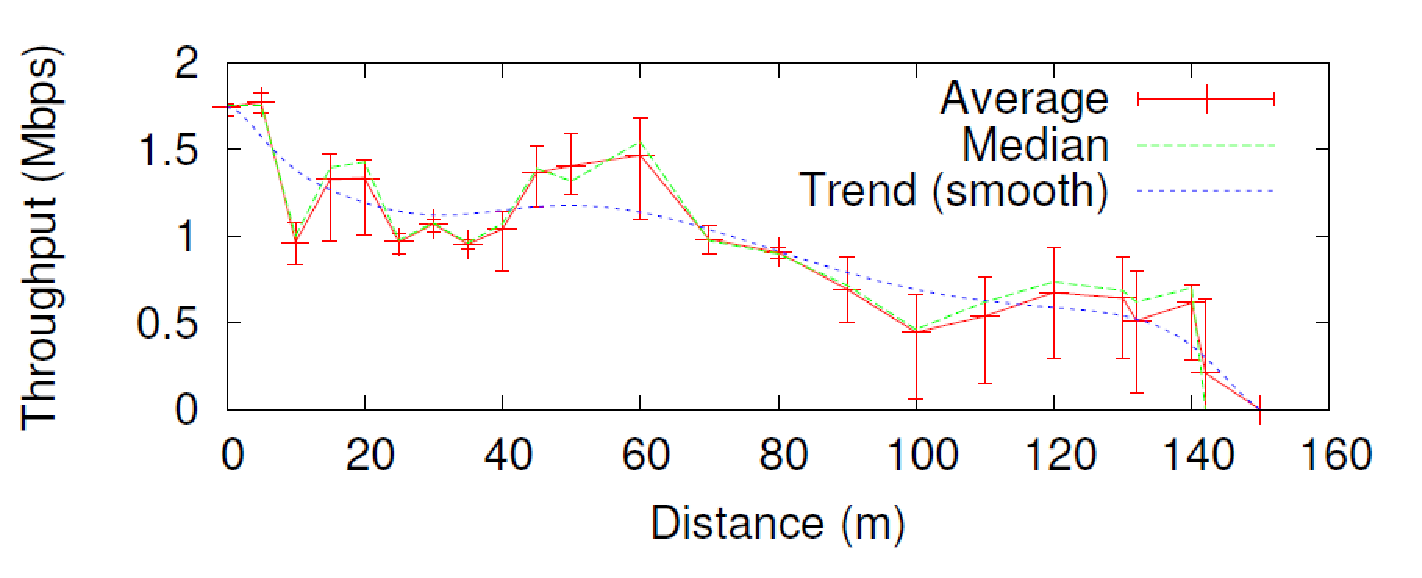
\includegraphics[width=0.7\textwidth]{images/btin.pdf}
	}\par\medskip
	\subcaptionbox{Throughput in indoor with obstacles.\label{fig:btobs}}{
		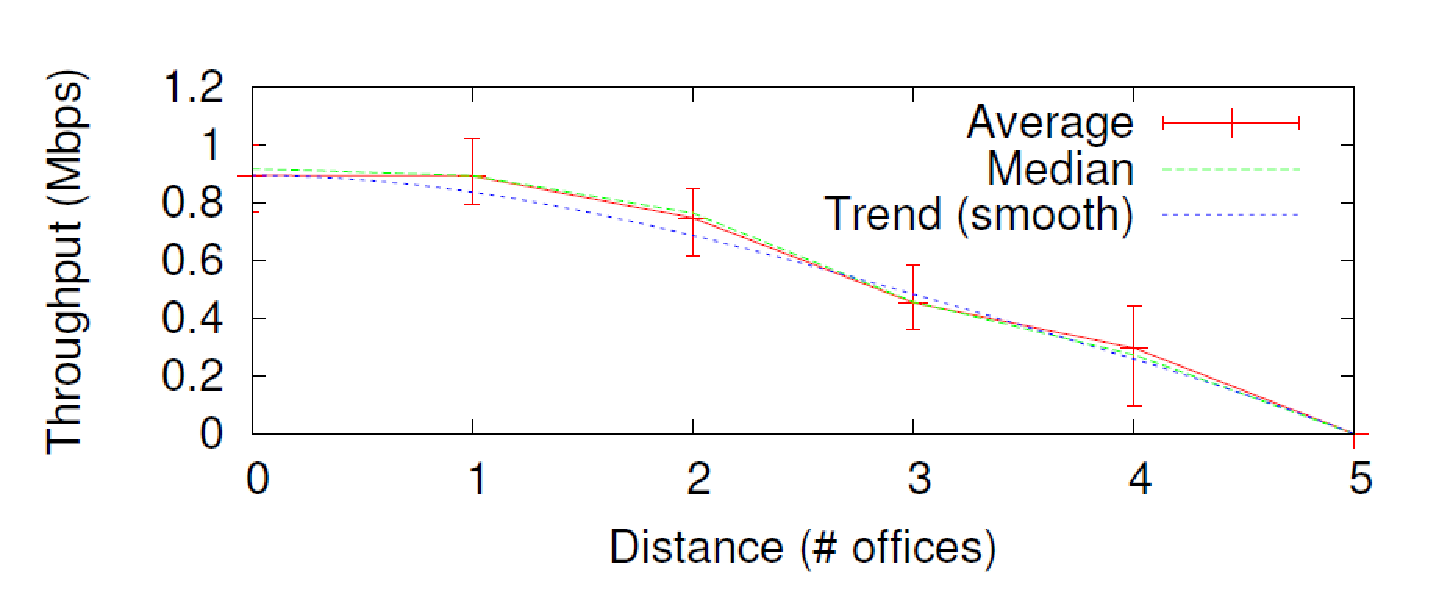
\includegraphics[width=0.7\textwidth]{images/btobs.pdf}
	}\par\medskip        
	\subcaptionbox{Throughput in outdoor line-of-sight.\label{fig:btout}}{
		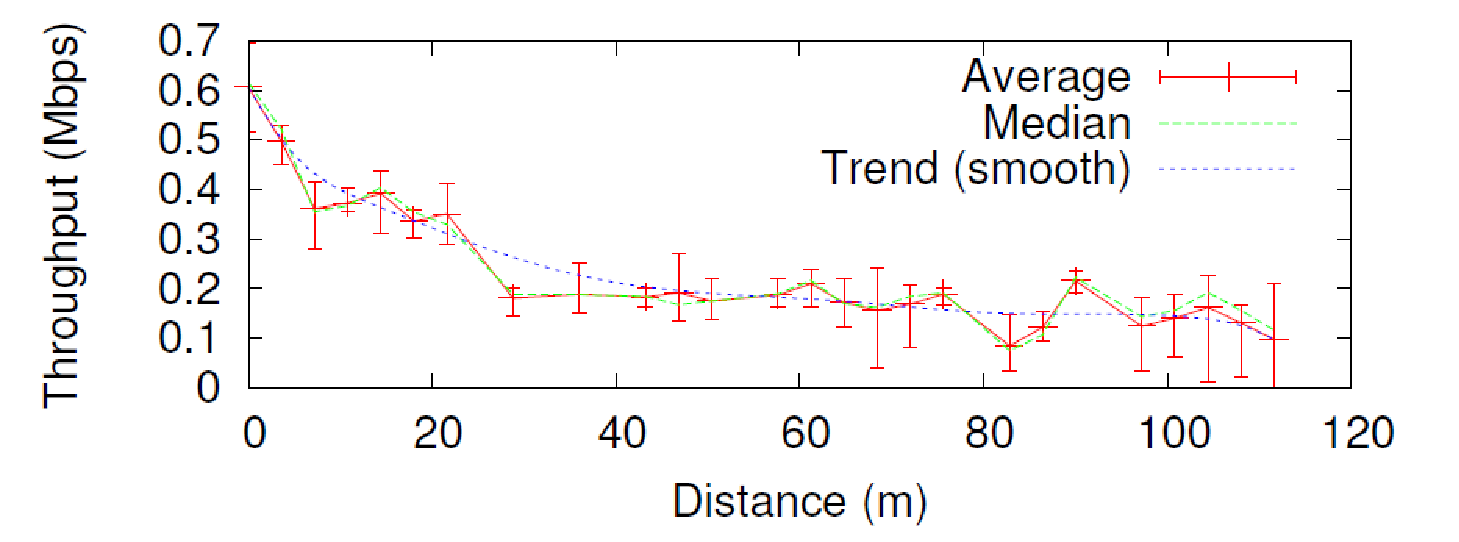
\includegraphics[width=0.7\textwidth]{images/btout.pdf}
	}
	\caption{Android Bluetooth single-hop throughput measurements in different environments (source \cite{throughputpaper}).}
	\label{fig:btthroughput}
\end{figure}

Overall, the devices using Bluetooth were able to communicate from \textit{20m} with obstacles, similarly to what was observed in \ref{subsec:ranges}, to \textit{150m} in the indoor line-of-sight environment. This disparity in the Bluetooth coverages comes from the phenomenon of signal reflections in the indoor environment, increasing the Bluetooth signal and consequently, its range. The throughput varied from \textit{0.6Mbps}, in the outdoor line-of-sight environment, to \textit{2.0Mbps}, in the indoor line-of-sight environment. This difference may be due to the channel interference, more prone to occur in the outdoor environment. 

Comparing the obtained measurements with the theoretical values, it can be said that (1) the throughput was significantly lower than what was stipulated in \cite{bluetoothspec}. Although, \gls{TCP} packets were used to measure the throughput, which may incur into further delays, as mentioned by the authors; (2) the communication ranges were much higher than the theoretical stipulation of \textit{10m} for Class 2 devices, which most smartphones are - see \cite{bluetoothspec}. However, for higher communication ranges, the throughput is much smaller, sometimes almost null, as seen in Figure \ref{fig:btout}.

In Figure \ref{fig:wfthroughput}, it is possible to see the measured throughput of the devices, when communication via Wi-Fi. The authors state that, even though the showed results are obtained using Wi-Fi, the conclusions can be drawn to Wi-Fi Direct, as the results are "redundant".

Figure \ref{fig:wfin} represents a plot of the measured throughput in the indoor line-of-sight environment. At a distance of \textit{0m}, the maximum throughput of \textit{40Mbps} is achieved. It then linearly decreases until a distance of \textit{125m}, where the throughput is almost null. At a distance of \textit{200m} the throughput is, roughly, \textit{1Kbps}.

Figure \ref{fig:wfobs} shows the measured throughput in the indoor with obstacles environment. At a distance of \textit{0m}, the measured throughput is \textit{30Mbps}. The indoor with obstacles environment presents a similar throughput decay as the one presented in Figure \ref{fig:wfin}. At a distance of 4 offices (\textit{100m}), the throughput measured less than \textit{5Mbps}.

In Figure \ref{fig:wfout}, the measured throughput in the outdoor line-of-sight environment is shown. At a distance of \textit{0m}, the throughput measures \textit{35Mbps}. However, at a distance of \textit{50m}, it measured less than \textit{5Mbps}. Despite what happened in the two previous environments, in the outdoor line-of-sight environment, the throughput decayed exponentially with the distance. At a distance of \textit{200m}, the throughput reaches \textit{0.8Mbps}, a much higher value than the one registered in the indoor line-of-sight environment.

\begin{figure}[ht]
	\centering
	\subcaptionbox{Throughput in indoor line-of-sight.\label{fig:wfin}}{
		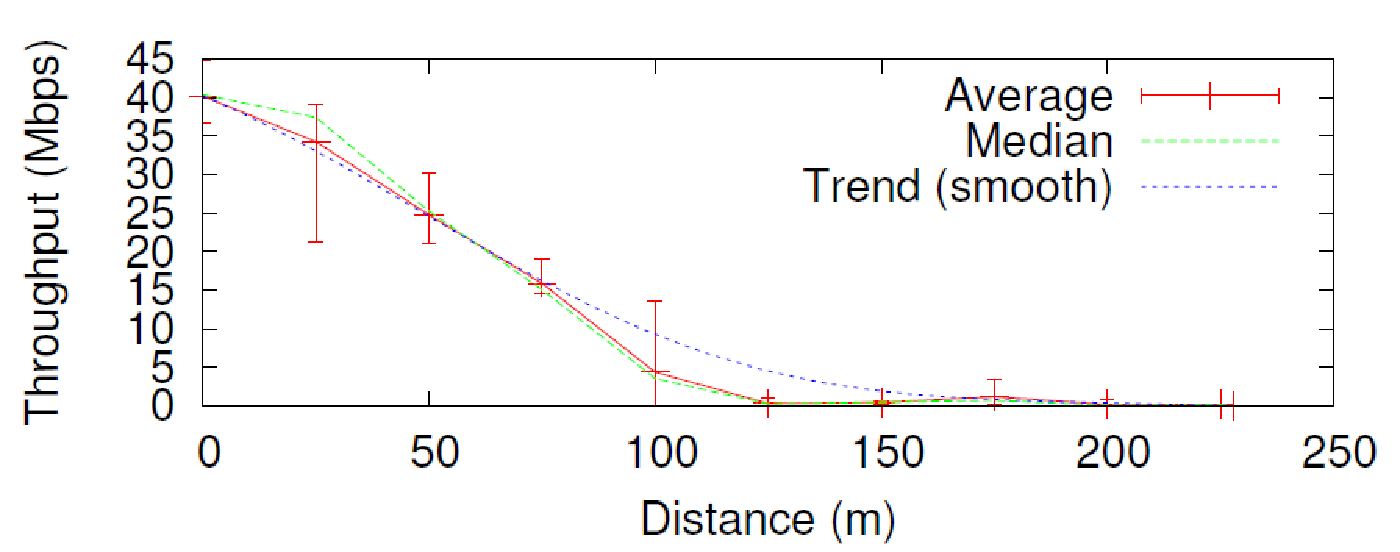
\includegraphics[width=0.7\textwidth]{images/wfin.pdf}
	}\par\medskip
	\subcaptionbox{Throughput in indoor with obstacles.\label{fig:wfobs}}{
		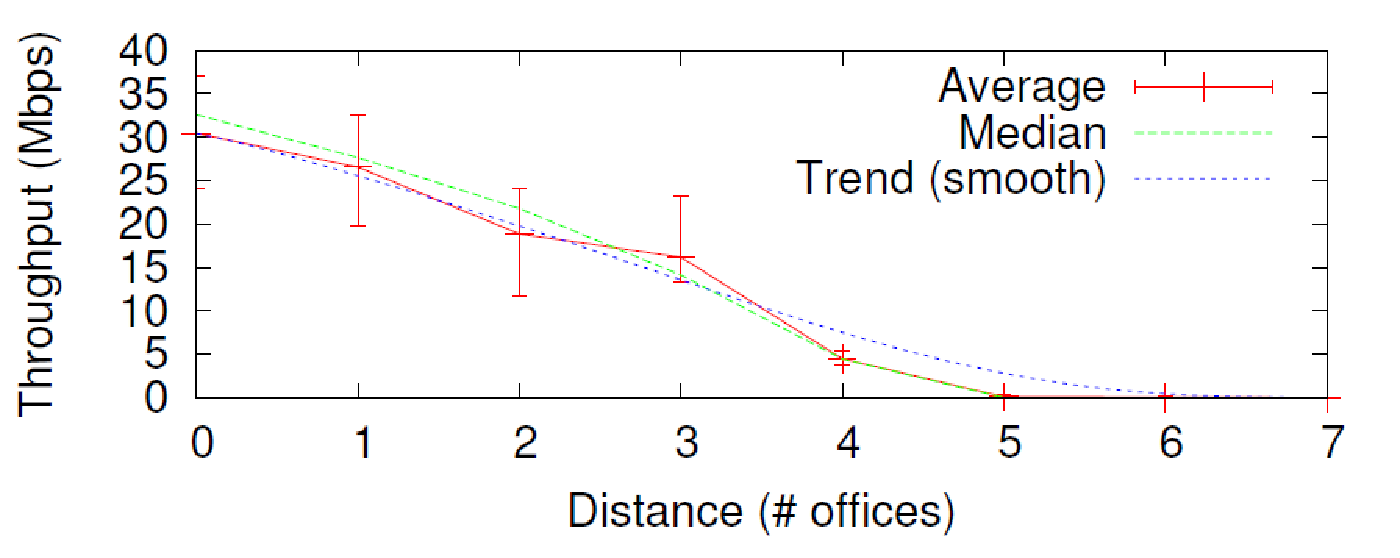
\includegraphics[width=0.7\textwidth]{images/wfobs.pdf}
	}\par\medskip        
	\subcaptionbox{Throughput in outdoor line-of-sight.\label{fig:wfout}}{
		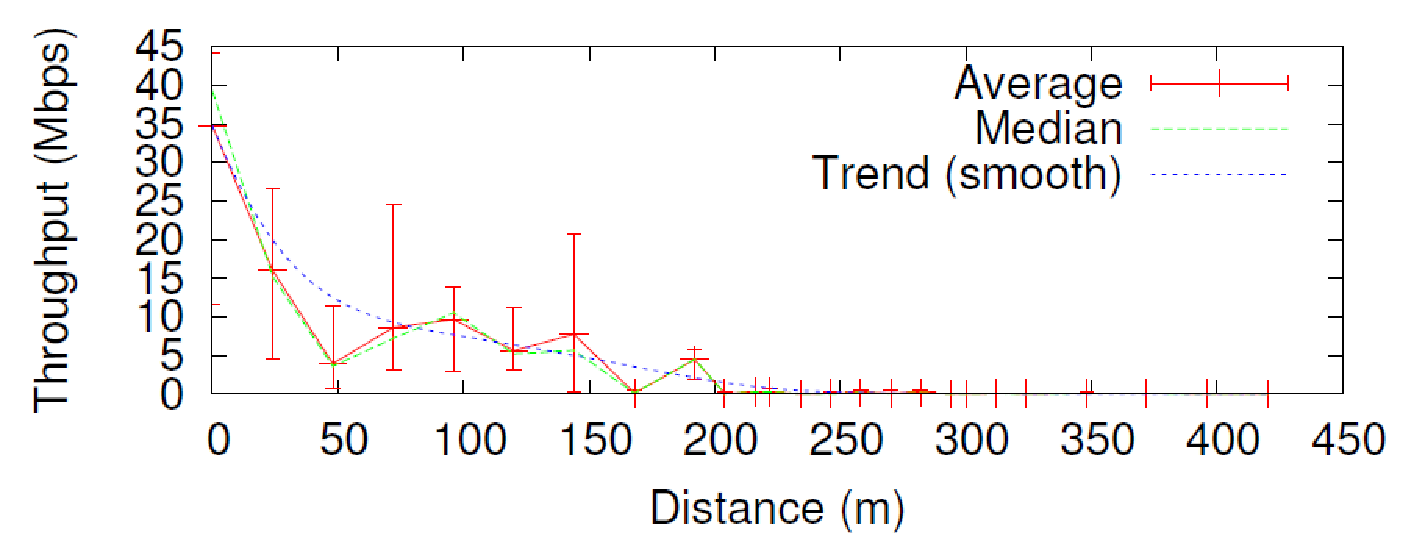
\includegraphics[width=0.7\textwidth]{images/wfout.pdf}
	}
	\caption{Android Wi-Fi single-hop throughput measurements in different environments (source \cite{throughputpaper}).}
	\label{fig:wfthroughput}
\end{figure}

After the brief analysis of the shown plots, it is possible to say that the indoor line-of-sight and indoor with obstacles environment present a similar throughput trend (in blue). In the outdoor line-of-sight environment, however, the throughput decays faster, in an exponential manner. This difference is due to the fact that "(...) propagation delay spreads are much smaller in indoor environments than outdoor environments.", taken from \cite{throughputpaper}. Having bigger delays, some reflections of the signal do not reach the server device during the \textit{2s} measured intervals, reducing the throughput.

However, at distances bigger than \textit{200m}, outdoor environments show a much higher throughput than indoor environments. This is due to the fact that reflected and scattered signals are cancelled by signal attenuation, highly reducing the throughput and, as mentioned before, the reflection and scattering phenomena are more relevant in indoor environments.

It is also possible to state that, in no experiment, the throughput reached the theoretical value of \textit{250Mbps}. The maximum throughput measured was in the indoor line-of-sight environment with a value of \textit{40Mbps}, less than a fifth of the maximum theoretical value.

\section{Testing the Developed Application}

In this section several tests will be executed, aiming to provide an overview of the developed application's performance. A conclusion will be given, reflecting on where the application performs the best and worse.

\subsection{Discovery Times}
\label{subsec:appdisc}

In this subsection the developed application discovery times will be tested. To obtain a meaningful analysis, the devices used are the same as the ones used in Subsection \ref{subsec:normaldisc}. It is expected that the measured discovery time values don't differ greatly from the ones previously obtained in Subsection \ref{subsec:normaldisc}.

Once again, the discovery times are measured in the same conditions as in Subsection \ref{subsec:normaldisc} and the number of discovered peer devices ranges from 0 to 2 devices found. However, to retrieve the Bluetooth discovery times the Android debugger was used, providing a precision of \textit{0.5ms}.

In Figure \ref{fig:appdisc}, the times measured during the developed application's discovery are shown, alongside the theoretical value of \textit{10.24s}, mentioned in Subsection \ref{subsec:normaldisc}.

Analysing the plot it is possible to see that (1) Samsung Grand Neo (in blue) shows the best Bluetooth discovery times, being almost constant throughout the sample space. It provides an average discovery time of \textit{12.826s}; (2) Motorola Moto G2's (in green) discovery times were similar to Samsung Grand Neo's discovery times, except for punctual samples, where the times are slightly bigger. It provides an average discovery time of \textit{12.991s}; (3) Huawei P8 Lite (in purple) provides the most irregular measures, similarly to what happened in Subsection \ref{subsec:normaldisc}. Its measured times range from \textit{15s} to \textit{18s}, having an average of \textit{16.755s}.

\begin{figure}[ht]
	\noindent\makebox[\textwidth]
	{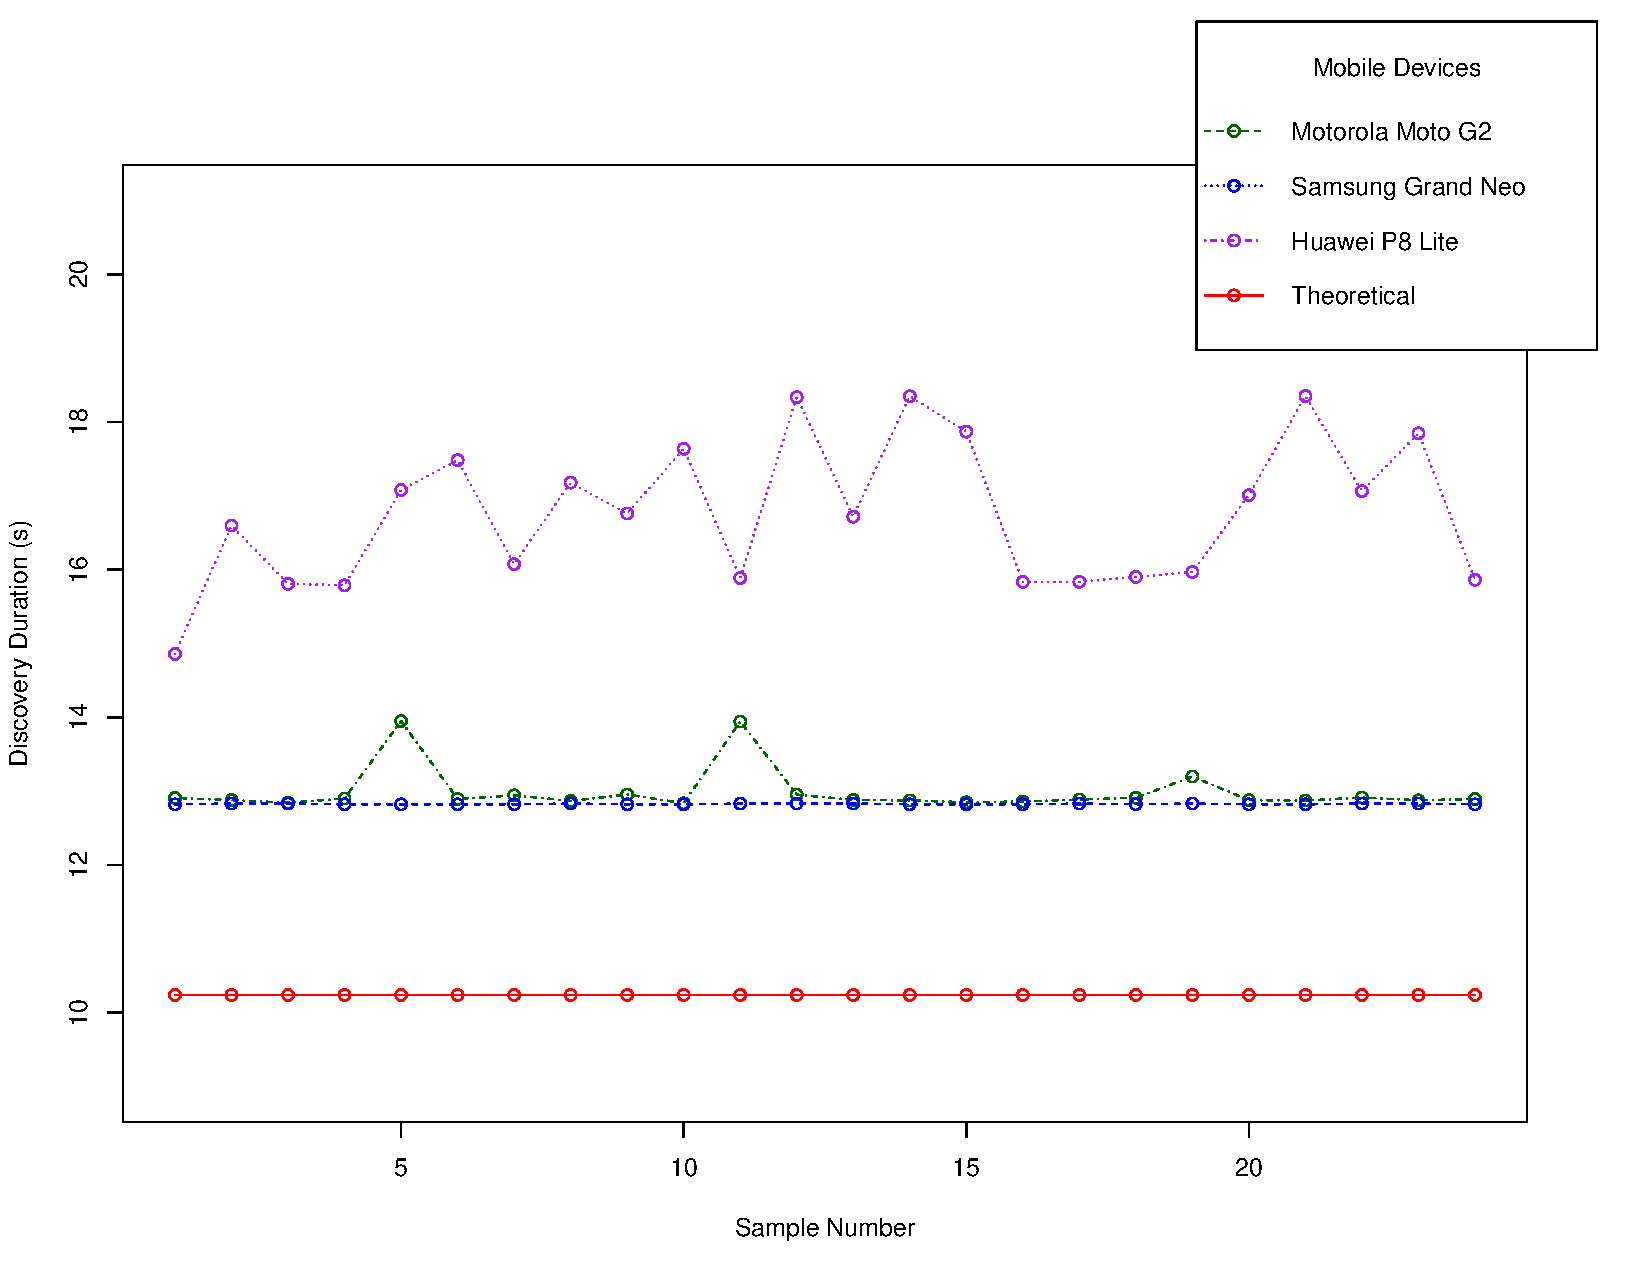
\includegraphics[width=1.2\textwidth]{images/plot_app_disc.pdf}}
	\caption{\label{fig:appdisc} Plot of the Bluetooth discovery times measured while using the developed application from the three devices.}
\end{figure}

As expected, the measured application discovery times were very similar to the ones obtained during a native discovery time. All the devices maintained the same properties they presented in \ref{subsec:normaldisc}: Samsung Grand Neo was mostly constant in both tests, providing the lowest discovery times; Motorola Moto G2 provided the second best discovery times, showing less deviation from the average in the current test than during the test performed in \ref{subsec:normaldisc}; Huawei P8 Lite showed the worst discovery times, however its average discovery time was similar in both tests. It also showed the most deviation from the average in both tests, having a bigger amplitude of results in the current test, as mentioned before.

Once again, it is possible to see that all three devices failed to meet the theoretical value of \textit{10.24s}, having shown discovery time averages of the theoretical time plus \textit{2s} to \textit{4s}.

\subsection{Advertisement Times}

In this subsection the advertisement times will be measured and analysed. There will be two sets of tests: one where devices advertise to one peer and another one where devices advertise to two peers. These two sets of tests aim to provide a better understanding on how much time the advertisement process occupies during an application run.

The devices used to test the advertisement process duration are the same used in the previous test: Motorola Moto G2, Samsung Grand Neo and Huawei P8 Lite. Since the application needs to establish a connection per peer device found, it is expected that the advertisement times to one peer will be slightly lower than the advertisement times to two peers, although the difference should not impact the overall application runtime.

In Figure \ref{fig:adv1} it is possible to see a boxplot of the advertisement times of the three devices. Analysing the boxplot it is possible to see that (1) Motorola Moto G2 has the lowest average advertisement time, as well as the lowest standard deviation from the three devices. It provides, approximately, a maximum of \textit{2s} and a minimum of \textit{0.75s}, having an average advertisement time of \textit{1.333s}; (2) Unlike the tests in Subsection \ref{subsec:appdisc}, Samsung Grand Neo has the biggest standard deviation, covering the biggest and smallest advertisement time values from the three devices. It provides, approximately, a maximum advertisement time of \textit{3.5s} and a minimum of \textit{0.35s}, having an average advertisement time of \textit{1.514s}; (3) Huawei P8 Lite has most of its values in the interval between \textit{1.75s} and \textit{1s}. It provides, approximately, a maximum of \textit{2s} and a minimum advertisement time of \textit{0.75s}, having an average advertisement time of \textit{1.388s}.

\begin{figure}[ht]
	\noindent\makebox[\textwidth]
	{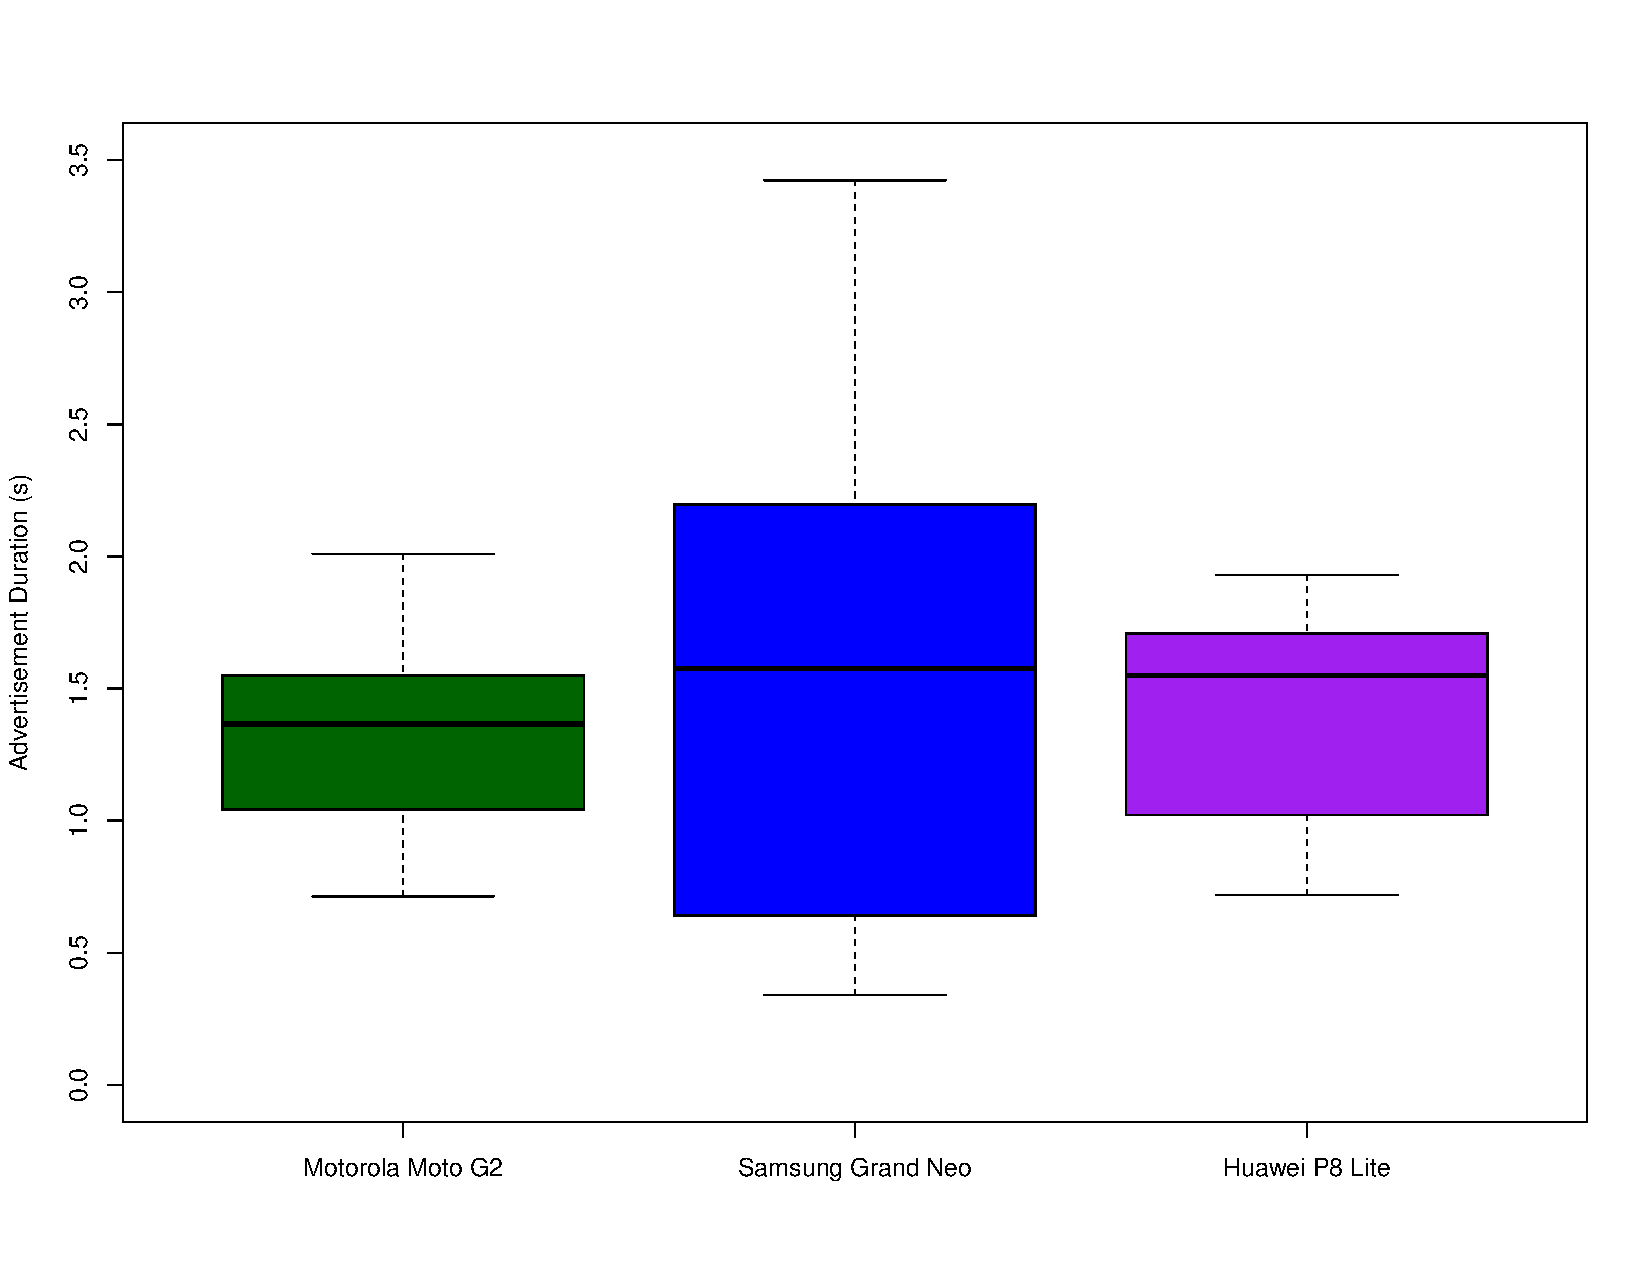
\includegraphics[width=1.2\textwidth]{images/boxplot_adv_1.pdf}}
	\caption{\label{fig:adv1} Boxplot of the advertisement times to one peer measured while using the developed application from the three devices.}
\end{figure}

All three tested devices provide a similar average advertisement time. In the next test, these devices will advertise to two distinct peers. In Figure \ref{fig:adv2}, it is possible to see a boxplot of thee advertisement durations of the three tested devices. It is also visible, that the disparity between durations is significantly higher than in the previous experiment, due to the supplementary complexity of advertising to more than one peer and establishing the individual connections.

In the boxplot of Figure \ref{fig:adv2}, it can be seen that (1) Motorola Moto G2's advertisement times range from, approximately, \textit{1.8s} to \textit{5.2s}, having an average advertisement time of \textit{3.066s}. In comparison with the previous test, the amplitude of advertisement durations is now of around \textit{3.4s}, compared to the previous \textit{1.25s}; (2) Samsung Grand Neo, similarly to the previous test, shows the biggest disparity of results, ranging from \textit{1.7s} to \textit{7s}, approximately, also having a bigger results amplitude of \textit{6.3s}, than previously measured \textit{3.15s}. It provides an average advertisement time to two peers of \textit{3.449s}; (3) Huawei P8 Lite shows the smallest standard deviation, having measures ranging from \textit{2.2s} to \textit{4.1s}. This device provides an average advertisement time to two peers of \textit{3.414s}.

\begin{figure}[ht]
	\noindent\makebox[\textwidth]
	{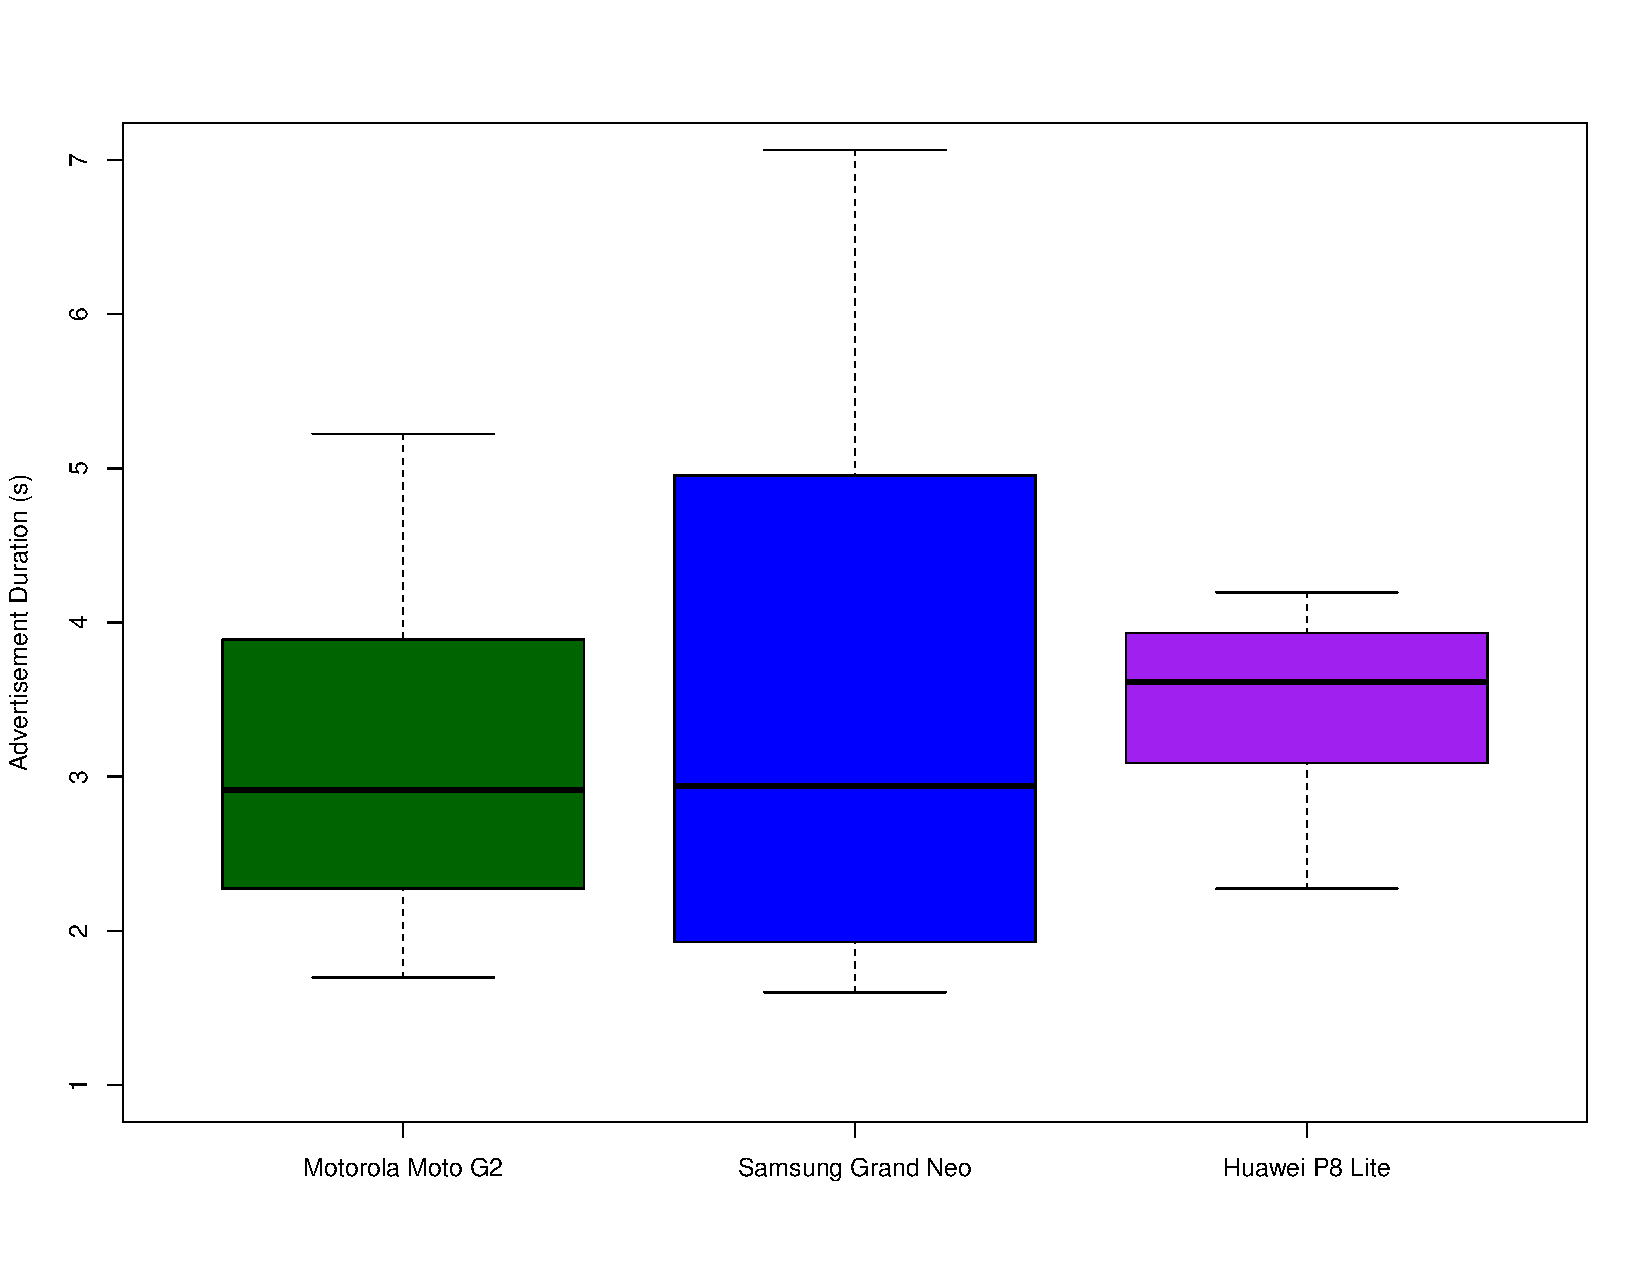
\includegraphics[width=1.2\textwidth]{images/boxplot_adv_2.pdf}}
	\caption{\label{fig:adv2} Boxplot of the advertisement times to two peers measured while using the developed application from the three devices.}
\end{figure}

Reflecting on the results of these two experiments, it is plausible to say that, despite the different behaviours, a similar average advertisement time was measured in the three devices, in both experiments. The advertisement times between experiments were a bit different, as was expected. Since individual connections must be established between advertiser and its peers, the first experiment sets the base advertisement time, as it reflects a one-to-one advertisement. The second experiment reflects a one-to-two advertisement and, the measured average times are double the one-to-one advertisement times, approximately.

A possible, valuable conclusion that may be taken from these tests is that the advertisement time is given by, approximately, the base advertisement time times the number of peers being advertised to. Although this is not confirmed, due to lack of testing equipment.

\subsection{Web Page Exchange Throughput}

In this subsection the web page exchange data rates will be measured and analysed. Moreover, to better understand where the developed framework and application are investing the most time, an analysis on the percentage of time spent in each process, during the web page exchange, will be shown.

To measure the throughput and percentage of time spent by each process, during the web page exchange, four environments were used: the first was using two devices, one acting as client and another one acting as server, similar to what was shown in Figure \ref{fig:adveg1}, being transferred a web page with \textit{1.911KB} (\url{https://www.example.com}). The second environment maintained the network topology, with two devices however, the transferred web page was larger, containing \textit{105.5KB} (\url{https://www.google.com}). The third environment used three devices, one acting as client, one as relay node and one as server, similar to the topology shown in Figure \ref{fig:example1.0}, the transferred web page was the same as in the first experiment. The last experiment used the same topology as before however, the transferred web page corresponded to the one used in the second environment, with \textit{105.5KB}.

Before analysing the plots, it is important to understand what processes are present in the web page exchange, described in Subsection \ref{subsec:exch}, and how was the throughput measured. Since there are two different network topologies, there will be different processes to be analysed, depending on the experiment.

In the two first experiments, two devices are used, meaning (1) one request is issued from the client to the server (\textit{Request \#1}); (2) the web page is downloaded (\textit{Download Web Page}); (3) the response is sent from the server to the client (\textit{Response \#1}); (4) the web page is transferred from the server to the client (\textit{Web Page Transfer \#1}).

In the third and fourth experiments, three devices are used, meaning (1) a request from the client to the relay node is sent (\textit{Request \#1}); (2) the request is forwarded from the relay to the server node (\textit{Request \#2}); (3) the web page is downloaded (\textit{Download Web Page}); (4) a response is sent from the server to the relay node (\textit{Response \#1}); (5) the web page is transferred from the server to the relay node (\textit{Web Page Transfer \#1}); (6) the reponse is forwarded from the relay node to the client (\textit{Response \#2}); (7) the web page is transferred from the relay node to its final destination (\textit{Web Page Transfer \#2}).

To measure the throughput in the first and second environments, the number of transferred bits of the web page are divided by the number of seconds that the application took to accomplish the following processes: \textit{Response \#1} and \textit{Web Page Transfer \#1}.

In the third and fourth environments, the throughput was measured by dividing the transferred web page bits by the number of seconds that the application took to conclude the processes of: \textit{Response \#1}, \textit{Web Page Transfer \#1}, \textit{Response \#2} and \textit{Web Page Transfer \#2}.

The \textit{Download Web Page} and previous processes were not taken into account, when measuring the throughput, as their durations are dependent on the server node's Internet connection quality.

In Figure \ref{fig:boxplotthroughput}, the measured throughputs in the previously described environments are shown. In the first and third environments, the average throughput is similar, around \textit{0.3Mbps}. Also, if compared to the other two environments, it is possible to see that the standard deviations are bigger, this is mainly due to the small duration of the web page exchange, making the measuring harder and less precise. The second and fourth environments provide similar results, with an average throughput of, roughly, \textit{0.75Mbps} and little standard deviation.

\begin{figure}[ht]
	\noindent\makebox[\textwidth]
	{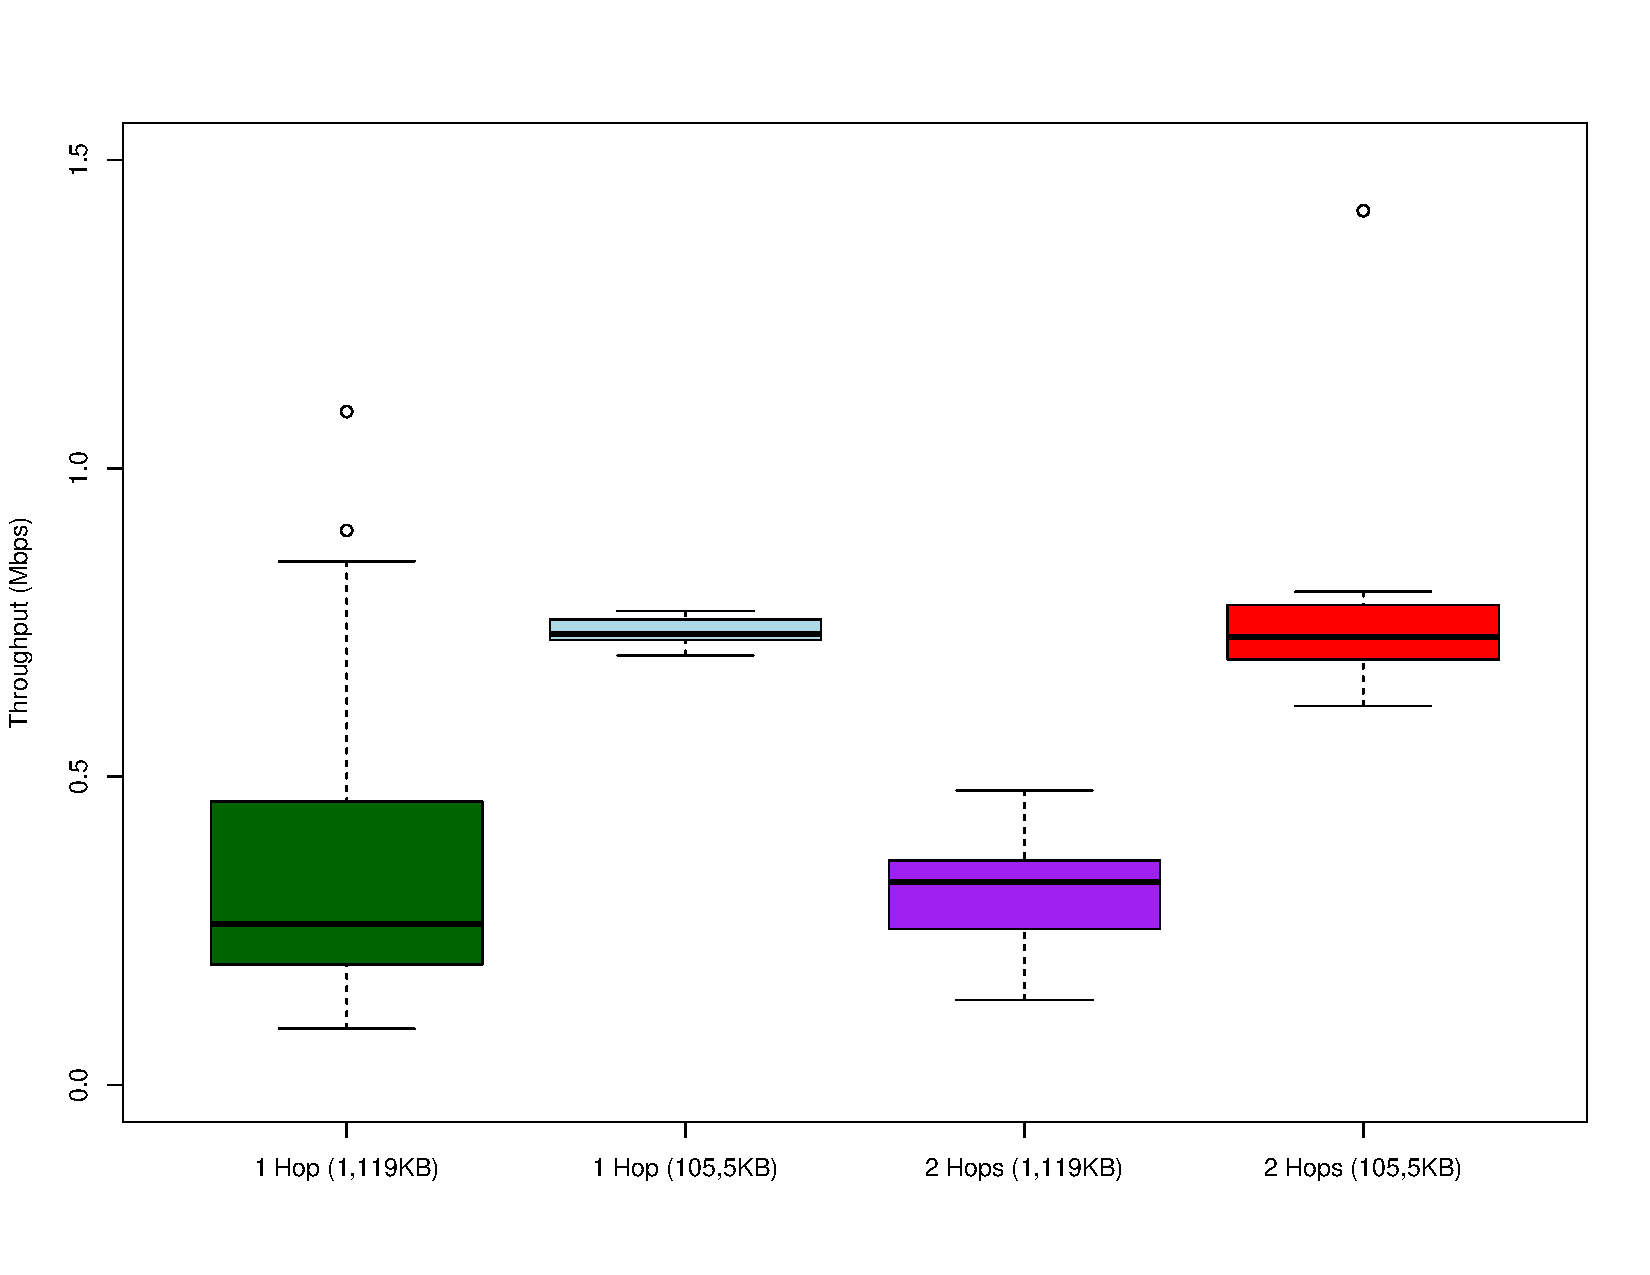
\includegraphics[width=1.2\textwidth]{images/boxplot_throughput.pdf}}
	\caption{\label{fig:boxplotthroughput} Boxplot of the measured throughput in the different experiment environments.}
\end{figure}

The results seen in Figure \ref{fig:boxplotthroughput} are to be expected since, when exchanging smaller web pages, the connection and application specific computation delays, such as the queries to the Response Table to retrieve the next hop and the analysis of the received data, have a more significant impact in the overall delay of process than when exchanging larger web pages. Hence, the lower average throughput measured in the first and third environments and bigger average throughput in the remaining environments.

If compared to the results shown in Subsection \ref{subsec:normalftdr}, the measured throughputs are smaller, than the Bluetooth indoor line-of-sight throughput measured at a distance of \textit{0m}. In this experiment, the maximum average throughput obtained was of, approximately, \textit{0.75Mbps}, a value lower than the \textit{2Mbps}, seen in Figure \ref{fig:btin}. This difference is again justified with the delays introduced by the connections and application specific computations during the exchange of web pages.

To measure the percentage of time spent by each of the processes, described above, during a web page exchange, the duration of that process was divided by the total duration of the web page exchange, since the initial request is sent until the final web page is received by the destination.

In Figure \ref{fig:perctime}, a barplot is presented, showing the different percentages of time each process took, in each environment. Starting from left to right (first to last environment), it is possible to see that (1) in the first environment the majority of time was spent downloading the web page, representing over \textit{70\%} of the total duration. The remaining processes' durations sum up to less than \textit{10\%} of the total duration; (2) the second environment shows that two processes occupy most of the total duration, \textit{Download Web Page} and \textit{Web Page Transfer \#1}. Combined, they sum more than \textit{90\%} of the total duration, representing roughly \textit{50\%} and \textit{40\%} of the web page exchange's duration, respectively. The remaining processes are, almost, insignificant in the overall duration of the web page exchange; (3) the third environment shows a similar process distribution to the first environment, with the \textit{Download Web Page} process occupying significantly more than the rest of the process, around \textit{30\%}. It is also seen that, despite more processes being measured, the total duration of the processes reaches less than \textit{35\%} of the total duration; (4) in the fourth environment, the most time costly processes are: \textit{Download Web Page}, \textit{Web Page Transfer \#1} and \textit{Web Page Transfer \#2}. Together, they represent close to \textit{70\%} of the total duration. The remaining processes are insignificant, summing up to little more than \textit{1\%} of the total duration.

Figure \ref{fig:perctime} also shows that, in the first and third environments, where the web page is smaller, the majority of time is occupied downloading it, as the transfer between devices of such a small number of bytes is almost immediate. It is also possible to see that, in this environments, the percentage of time occupied by the measured processes is less than in the environments with the same topology but where a larger web page is transferred, due to the connections establishment and application specific computations delays occupying a larger portion of the web page exchange duration. In the second and fourth environments, these delays occupy a smaller portion of time, since the download and transfers of the web page are longer.

\begin{figure}[ht]
	\noindent\makebox[\textwidth]
	{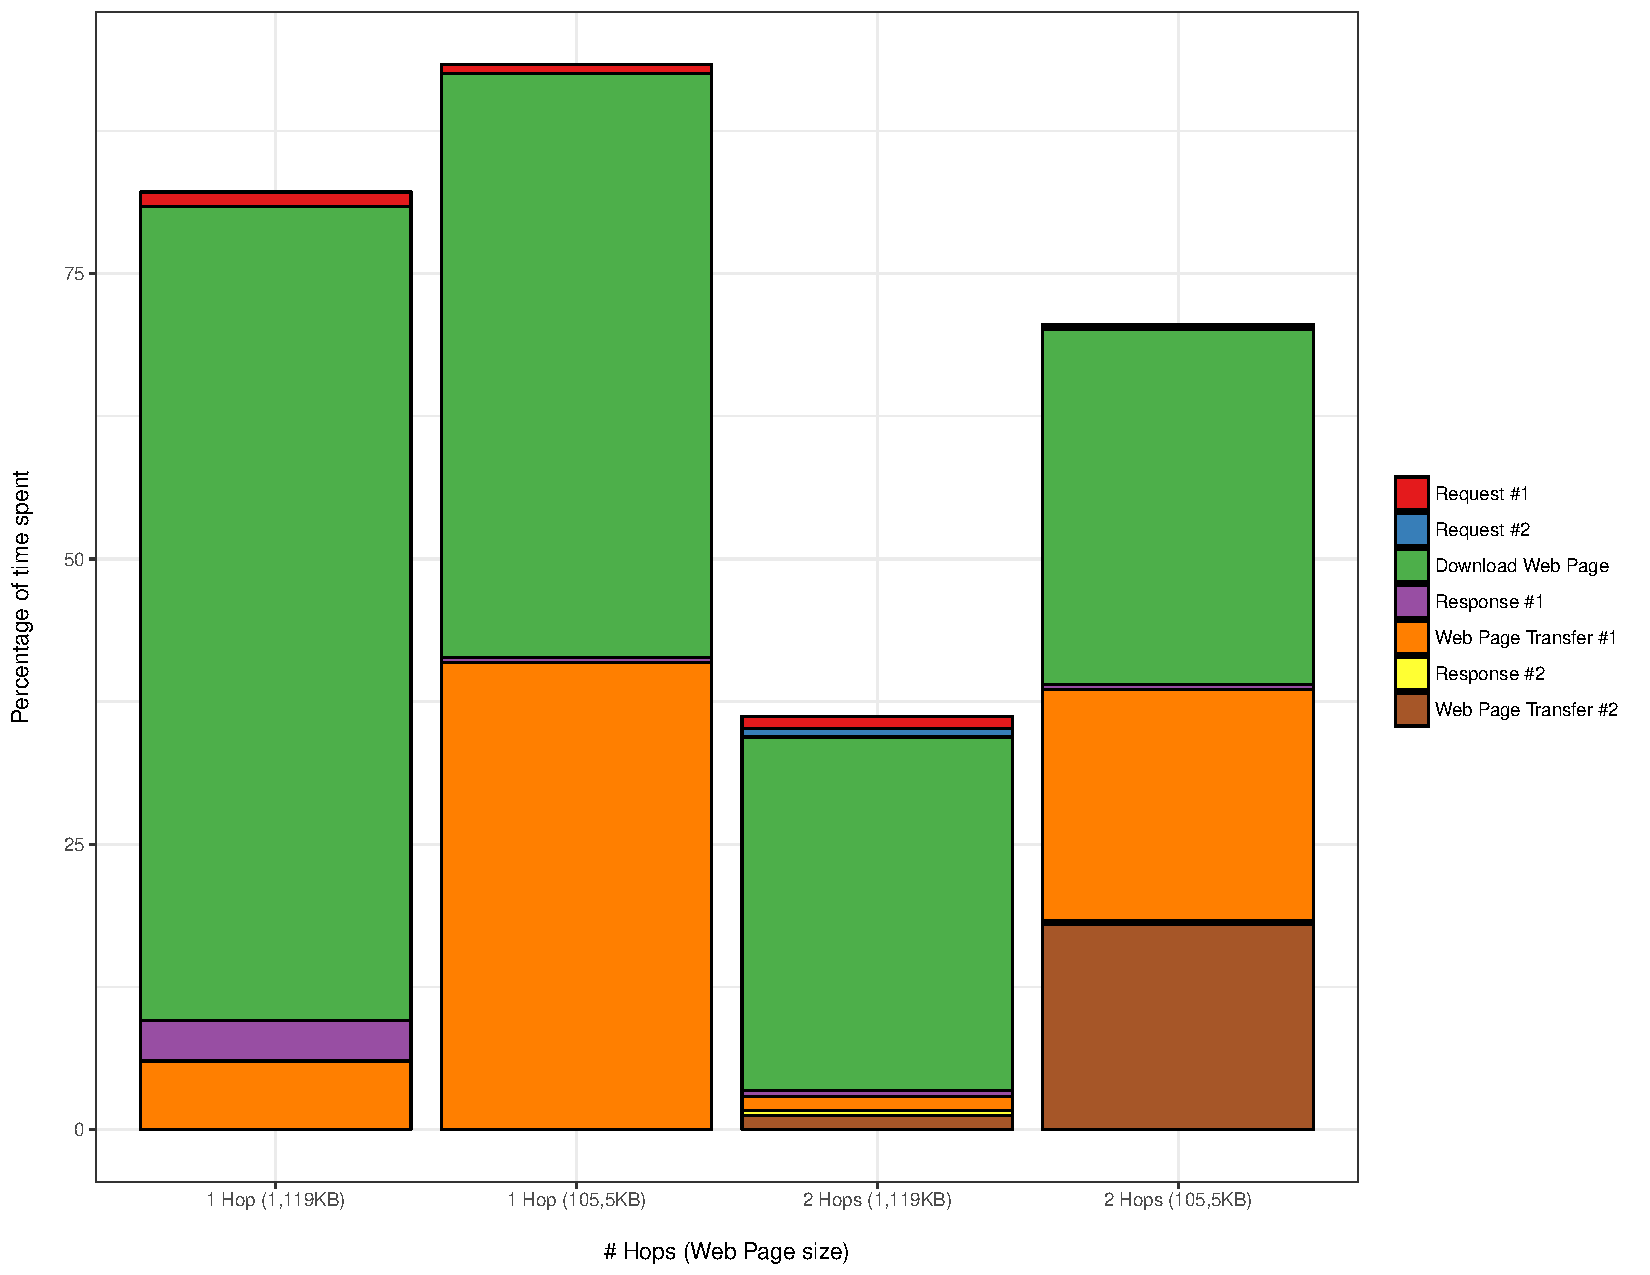
\includegraphics[width=1.2\textwidth]{images/barplot_perc_time.pdf}}
	\caption{\label{fig:perctime} Barplot of the percentage of occupied by the various processes in the different experiment environments.}
\end{figure}

As expected, when the web page size is bigger, so is the portion of time occupied by its transfer. The request and response sending processes are mostly insignificant, introducing little delay in the web page exchange process. Also as expected, in the third and fourth environment, the \textit{Web Page Transfer \#1} and \textit{Web Page Transfer \#2} processes occupy a similar percentage of the web page exchange duration, as the same number of bytes is being sent over a similar connection link.

As mentioned before, these results are influenced by the server node's Internet connection quality, impacting the duration the \textit{Download Web Page} process, especially when dealing with larger web pages. Despite that, the measured results are compatible to what was expected.




